\section{Vorlesung}

Ziel der Vorlesung: Studierende können univariate Analysen machen\\


\subsection{Datenmatrix}
\begin{itemize}
 \item auch \textit{Urliste} genannt
 \item Spalten $\rightarrow$ Variablen
 \item Zeilen  $\rightarrow$ Fälle
 \item Jeder Fall bekommt eine ID zugewiesen
\end{itemize}
==> Aufgabe 1 Serdar
\subsection{Häufigkeiten}
\textbf{f}requenz und \textbf{H}äufigkeit
\begin{itemize}
 \item [1.] \textbf{Absolute Häufigkeit:}~~ $fx_k = Hx_k$
 \item [2.] \textbf{Relative Häufigkeit:}~~ $\frac{fx_k}{n} = hx_k$
 \item [3.] \textbf{prozentuale Häufigkeit:}~~ $hx_k \cdot 100$
\end{itemize}

\subsection{kumulierte Häufigkeit}
politisches Interesse Allbus:\\
\begin{tabular}[h]{r|c|c|c|l}
        Kategorie   & $Hx_k$    &  $hx_k$   &  $hx_k \cdot 100$ & kumulierte prozentuale Häufigkeit  \\
  \hline
	sehr stark  & 425       & 0,122    & 12,2 & 12,2\\
        stark       & 877       & 0,251    & 25,1 & 37,3\\
        mittel      & 1437      & 0,412    & 41,2 & 78,5\\
        wenig       & 564       & 0,162    & 16,2 & 94,7\\
überhaupt nicht     & 186       & 0,053    & 5,3  & 100\\
  \hline
	Gesamt & 3490 & 1,000 & 100 & {}\\
\end{tabular}
\begin{enumerate}
\item Wie viele Menschen sind mindestens stark politisch interessiert? \solution{37,3\%}
\item Wie hoch ist der prozentuale Anteil der Personen, die weniger als <mittel> interessiert sind? \solution{$100\% - 37,3\% = 62,7\%$}
\item Wie hoch ist der prozentuale Anteil der Personen, <stark, mittel, wenig> angekreuzt haben? \solution{$94,7\% - 12,2\% = 82,5\% $}
\item Welche Häufigkeitsdarstellung zeigt am besten wie viele Individuen der Stichprobe vor dem 55. Lebensjahr in Rente gegangen sind? \solution{kumulative Häufigkeitsverteilung}
\end{enumerate}

\subsection{Darstellungsarten}
\begin{tabular}{r|l|l}
      {} & Variablenskala & zu beachten \\
\hline
Piechart & nominal        & nur wenig Kategorien\\
Säulendiagramm & nominal, ordinal & Reihenfolge auf X-Achse\\
Histogramm & intervall, ratio & hat Zweck Fläche darzustellen \textrightarrow Polygonzug/Dichteverteilung mit angeben  \\
\end{tabular}
\begin{figure}[h]
 \centering
 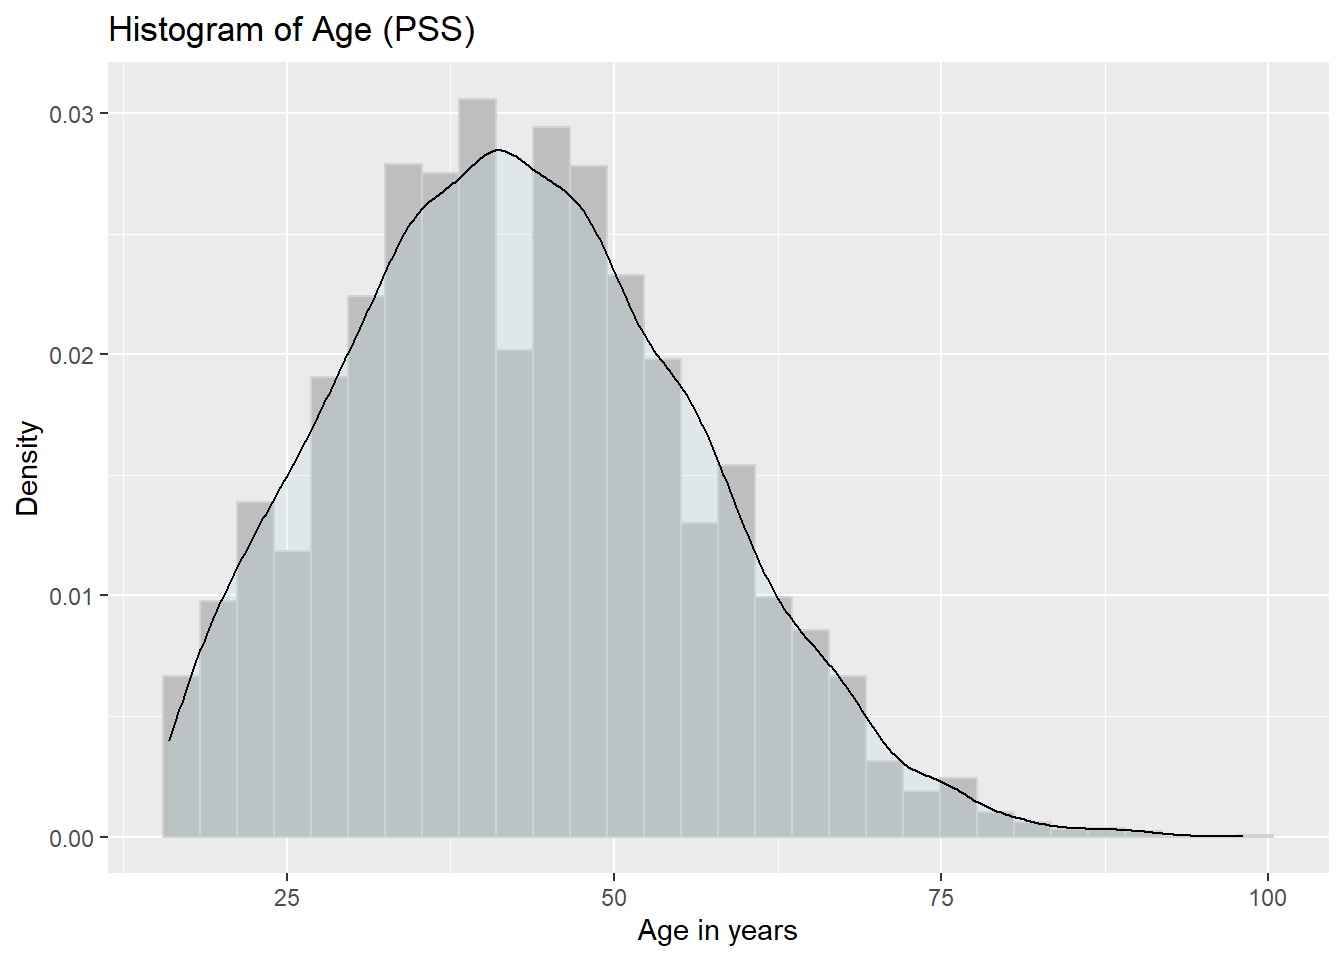
\includegraphics[scale=0.6]{./img/hist-density-1.png}
 \caption{Histogramm mit Dichteverteilung}
\end{figure}

\subsection{Verteilungsformen}
Symetrisch\\
Bimodal\\
linkssteil,rechtsschief\\
rechtssteil,linksschief\\
\\
\subsection{Summenzeichen}
$\sum_{i=m}^{n}a_i~~~=~~~a_{m} + a_{m+1} + a_{m+2} + a_{m+3} + \dots + a_{n}$
\\
Für alle Aufgaben gilt folgende Tabelle:
\begin{tabular}{c|ccccc}
    $\textrm{a}_\textrm{i}$ & $\textrm{a}_\textrm{1}$ & $\textrm{a}_\textrm{2}$ & $\textrm{a}_\textrm{3}$ & $\textrm{a}_\textrm{4}$ & $\textrm{a}_\textrm{5}$ \\ \hline
    x & 2 & 1 & 5 & 3 & 3
\end{tabular}

\begin{align*}
  A &= \sum_{i=1}^{n}x_{i}  &
  B &= \sum_{i=2}^{4}x_{i} &
  C &= \sum{x_{i}} &
  D &= \sum{x_{i}}^2 &
  E &= (\sum_{i=1}^{n}{x_{i}})^2 &\\\\
  F &= (\sum_{i=1}^{n}{x_{i}})-1 &
  G &= \sum_{i=1}^{n}(x_{i}-1) &
  H &= \sum_{i=1}^{n}(x_{i}-1)^2 &
  I &= (\sum_{i=1}^{n}(x_{i}-1))^2 &
  J &= \frac{\sum_{i=1}^{n}(x_{i}-1)}{n} &\\\\
  K &= \frac{\sum_{i=1}^{n}(x_{i}-2)^2}{n} &
  L &=  &
  M &=  &
  N &=  &
  O &=  &\\
\end{align*}
Lösungen:
\begin{tabular}{c|c|c|c|c|c|c|c|c|c|c|c|c|c|c}
    A  & B & C  & D  & E        & F  & G & H  & I        & J                 & K  & L  & M  & N  & O\\
    14 & 9 & 14 & 48 & $14^{2}$ & 13 & 9 & 25 & 81       & $\frac{9}{5}=1,8$ & $\frac{12}{5}$ & {} & {} & {} & {}
\end{tabular}
